\question[3]
Der Graph wird von Startknoten a aus mit Tiefensuche traversiert. Die
  Nachbarn werden in alphabetischer Reihenfolge besucht.
  Schreibe an die Knoten ihre previsit/postvisit Nummern.

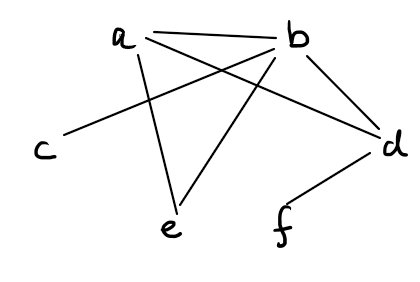
\includegraphics[height=5cm]{\pfad/Graphen/Aufgaben/visit_04/visit_04.png}

\ifprintanswers
Lösung:
\begin{lstlisting}
a  1 12
b  2 11
c  3  4
d  5  8
f  6  7
e  9 10
\end{lstlisting}
\fi
